
%----------------------------------------------------------------------------------------
%	Lecture 27
%----------------------------------------------------------------------------------------

\chapter{Stokes' Theorem} 

\bigbreak

\begin{mdframed}
\begin{center}
If $C$ is a closed curve in space then the line integral of a vector field ${\bf F}$ along $C$ can be given by
$$ \oint_{C} {\bf F} \cdot d{\bf r} = \iint_S (\nabla \times {\bf F}) \cdot \hat{n} dS $$
where $S$ can be any surface bounded by $C$ such that ${\bf F}$ is defined and differentiable everywhere on $S$.
\end{center}
\end{mdframed} 

\subsection*{Orienations} 

We need the orianations of $C$ and $S$ to be compatible.
The rule is :

If we walk along $C$ in the direction of its orientation with $S$ to the left then the normal vector is pointing up.

\begin{figure}[ht!]
    \centering
    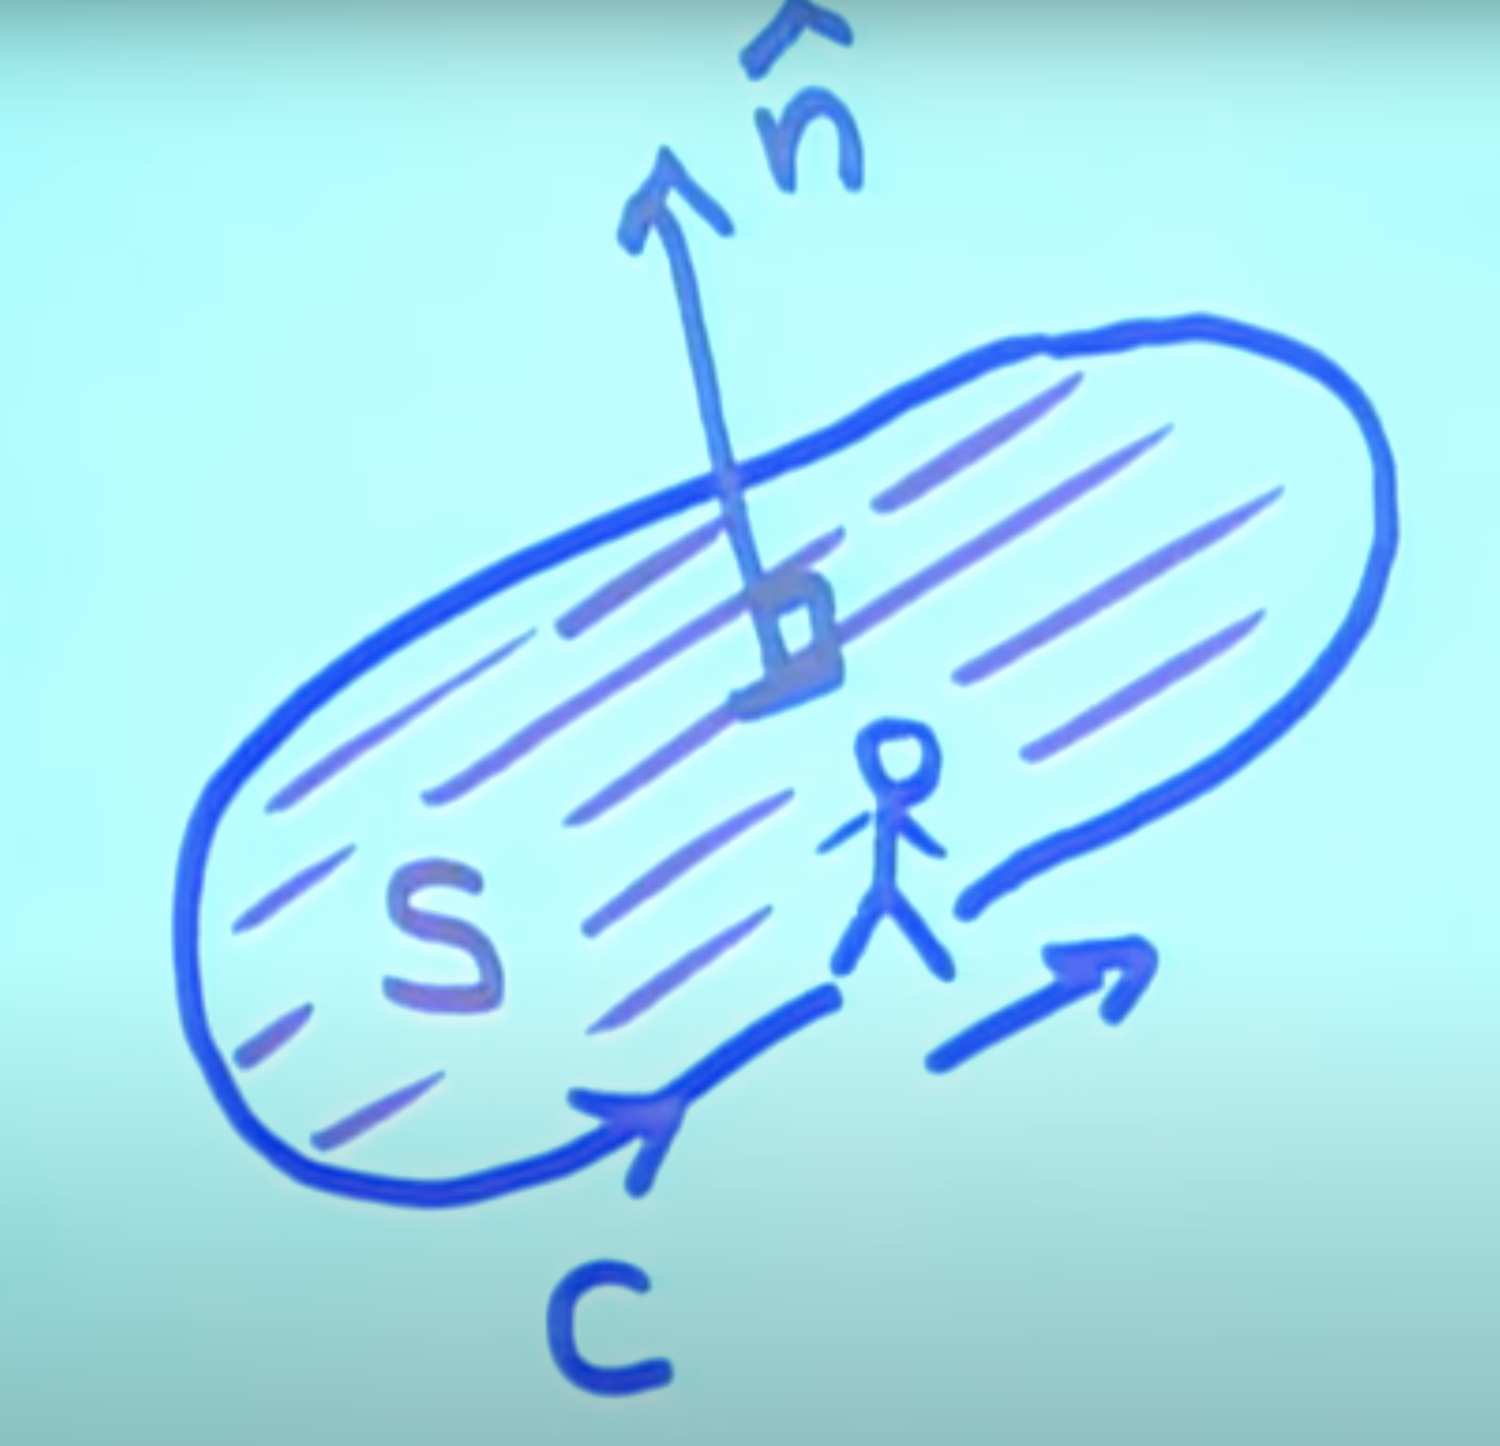
\includegraphics[scale=0.3]{./images/lecture_27_figure_1.png}
    \caption{Orianting Curve and Surface}
\end{figure}

Another way to do this is to use the right hand rule.
Point your thumg along the curve and point your index finger tangent the surface towards the interior of surface, 
then point your middle finger perpendicular to both and that will be the direction of the normal vector. 


\section{Comparing Stokes Theorem With Green's Theorem}

Let's say we have a closed curve lies in the $XY$-plane and goes in the counter clockwise direction.
And let $S$ be the surface in the $XY$-plane enclosed by $C$.
So if a vector field ${\bf F} = \left< P, Q, R \right>$ exists then 

$$ \oint_C {\bf F} \cdot d{\bf r} = \oint_C Pdx + Qdy $$

This is because we are in the $XY$-plane so $dz = 0$.
Now by Stokes' Theorem, 

$$ 
\oint_C {\bf F} \cdot d{\bf r} 
= \oint_C Pdx + Qdy 
= \iint_S (\nabla \times {\bf F}) \cdot \hat{n} dS 
$$

For our surface, the normal vector for our curve  will be $\hat{k}$. Now $(\nabla \times {\bf F}) \cdot \hat{k} = Q_x - P_y$
So, 

$$
\oint_C {\bf F} \cdot d{\bf r} 
= \oint_C Pdx + Qdy 
= \iint_S Q_x - P_y dS 
$$

This is exactly what Green's Theorem is. 
So Green's Theorem is just a special case of Stokes' Theorem in the $XY$-plane.


\section{Proof of Stokes' Theorem}

We will prove this the same way we proved Green's Theorem.

\begin{enumerate}
    \item Prove that the line integral of a vector field around a infinitesimal rectangle is equivalent to the curl times its area.
    \item Prove that we can combine rectangles with common edges and same orientation.
    \item Divided the surface into infinitesimal rectangles and sum them to find the total line integral.
\end{enumerate}

Here we will only do the first step because the second and third step have already been done in the proof for Green's Theorem.
And the first step is different here because the rectangle is in space instead of $XY$-plane.

Let's say our surface is given by a function $f(x, y, z) = 0$. 
So $df = f_x dx + f_y dy + f_z dz = 0$. 
Thus, \ilds{\diff{z}{x} = \frac{-f_x}{f_z}} and \ilds{\diff{z}{y} = \frac{-f_y}{f_z}}.

So let's say our rectangle is formed when we move by $dx \hat{i}$ and $dy \hat{j}$.
So our side vectors are $dx \hat{i} + dz \hat{k}$ and $dy \hat{j} + dz \hat{k}$.
We can substitute $dz$ from above equations as $dx \hat{i} - \frac{f_x}{f_z}\hat{k}$ and $dy \hat{j} - \frac{f_y}{f_z} dy \hat{k}$
So our area is $dS$ is cross product of these vectors which is 
$$
\hat{n} dS = \begin{vmatrix}
    \hat{i} & \hat{j} & \hat{k} \\
    dx & 0 & -\frac{f_x}{f_z} dx \\
    0 & dy & -\frac{f_y}{f_z} dy \\
\end{vmatrix} 
= \ijk{\frac{f_x}{f_z} dx dy }{\frac{f_y}{f_z} dx dy}{dx dy}
= ( \ijk{f_x}{f_y}{f_z} )\frac{dx dy}{f_z}
$$

Now the let's calculate the line integral. 
Our four endpoints will be  
$A(x, y, z)$, 
$B(x+dx, y, z - \frac{f_x}{f_z} dx)$, 
$C(x+dx, y+dy, z - \frac{f_x}{f_z}dx - \frac{f_y}{f_z} dy)$
and $D(x, y+dy, z - \frac{f_y}{f_z} dy)$.

\pagebreak

Let's say our vector field is ${\bf F} = \left< P, Q, R \right>$
Let's take our curve to be $ABCDA$. So our line integral becomes,


\begin{align*}
\oint_C {\bf F} d{\bf r} & = 
    \int_{AB} {\bf F} d{\bf r} +
    \int_{BC} {\bf F} d{\bf r} +
    \int_{CD} {\bf F} d{\bf r} +
    \int_{DA} {\bf F} d{\bf r} \\
    & = {\bf F}(x, y, z) \cdot 
        \left< dx, 0, - \frac{f_x}{f_z} dx \right> \\
    & + {\bf F}(x + dx, y, z - \frac{f_x}{f_z} dx) \cdot 
        \left< 0, dy, - \frac{f_y}{f_z} dy \right> \\
    & + {\bf F}(x + dx, y + dy, z - \frac{f_x}{f_z} dx - \frac{f_y}{f_z} dy) \cdot 
        \left< - dx, 0, \frac{f_x}{f_z} dx \right> \\
    & + {\bf F}(x, y + dy, z - \frac{f_y}{f_z} dy) \cdot 
        \left< 0, - dy, \frac{f_y}{f_z} dx \right> \\
    & = P(x, y, z) dx - R(x, y, z) \frac{f_x}{f_z} dx \\
    & + Q(x + dx, y, z - \frac{f_x}{f_z} dx) dy - R(x + dx, y, z - \frac{f_x}{f_z} dx) \frac{f_y}{f_z} dy \\
    & - P(x + dx, y + dy + z - \frac{f_x}{f_z} dx - \frac{f_y}{f_z} dy) dx 
        + R(x + dx, y + dy, z - \frac{f_x}{f_z} dx - \frac{f_y}{f_z} dy) \frac{f_x}{f_z} dx \\
    & - Q(x, y + dy, z - \frac{f_y}{f_z} dy) dy + R(x, y + dy, z - \frac{f_y}{f_z} dy) dy
\end{align*}

Let us combine the terms with $P$, $Q$ and $R$.

\begin{align*}
\oint_C {\bf F} d{\bf r} 
    & = (P(x, y, z) - P(x + dx, y + dy, z -  \frac{f_x}{f_z} dx - \frac{f_y}{f_z} dy)) dx \\
    & + (Q(x + dx, y, z - \frac{f_x}{f_z} dy) - Q(x, y + dy, z - \frac{f_y}{f_z} dy)) dy \\
    & + (R(x + dx, y + dy, z - \frac{f_x}{f_z} dx - \frac{f_y}{f_z} dy) - R(x, y, z) ) \frac{f_x}{f_z} dx \\
    & + (R(x, y + dy, z - \frac{f_y}{f_z} dy) - R(x + dx, y, z - \frac{f_x}{f_z} dx)) \frac{f_y}{f_z} dy
\end{align*}

Now we can apply linear approximation  to get simplify some of the terms.
Substuting these in the original equation, we get,

\begin{align*}
\oint_C {\bf F} d{\bf r} 
    & = ( - P_x dx - P_y dy + P_z \frac{f_x}{f_z} dx + P_z \frac{f_y}{f_z} dy ) dx \\
    & + (Q_x dx - Q_y dy - Q_z \frac{f_x}{f_z} dx + Q_z \frac{f_y}{f_z} dy) dy \\
    & + (R_x dx + R_y dy - R_z \frac{f_x}{f_z} dx - R_z \frac{f_y}{f_z} dy) \frac{f_x}{f_z} dx \\
    & + (R_y dy - R_x dx - R_z \frac{f_y}{f_z} dy + R_z \frac{f_x}{f_z} dx) \frac{f_y}{f_z} dy
\end{align*}

Now we can multiply everything out and simplify. 
Here we can ignore all the terms with $(dx)^2$ and $(dy)^2$ as they become zero as we take the limit.

\begin{align*}
\oint_C {\bf F} d{\bf r} 
    & = -P_y dx dy + P_z \frac{f_y}{f_z} dx dy \\
    & + Q_x dx dy - Q_z \frac{f_x}{f_z} dx dy \\
    & + R_y \frac{f_x}{f_z} dx dy - R_z \frac{f_x f_y}{f_z^2} dx dy \\
    & - R_x \frac{f_y}{f_z} dx dy + R_z \frac{f_x f_y}{f_z^2} dx dy \\
    & = (R_y - Q_z) \frac{f_x}{f_z} dx dy 
    + (P_z - R_x) \frac{f_y}{f_z} dx dy 
    + (Q_x - P_y)
\end{align*}


Now let's find the surface integral of $\nabla \times {\bf F}$.
We have $\hat{n} dS = \left< \frac{f_x}{f_z}, \frac{f_y}{f_z}, 1 \right> dx dy$
And, $ \nabla \times {\bf F} = \ijk{(R_y - Q_z)}{(P_z - R_x)}{(Q_x - P_y)}$

So the surface integral is 
$$
(\nabla \times {\bf F}) \cdot \hat{n} dS = 
(R_y - Q_z) \frac{f_x}{f_z} dx dy +
(P_z - R_x) \frac{f_y}{f_z} dx dy + 
(Q_x - P_y)
$$

Here, we can see that our line integral approximation is the same as the surface integral approximation.
So as we make the rectangles smaller these get equal.
And we can finally take the sum of all line integrals to find the line integral of a curve
and then we can integrate over the surface integral.